\documentclass[25pt, a0paper, portrait]{tikzposter}
\geometry{paperwidth=34in,paperheight=36in}

% Preamble
\title{Simulating Missile Trajectory with DEs}
\author{Colin Tierney}
\date{\today}
\institute{MTH3701 - Modeling + Simulation}
\usebackgroundstyle{Default}

% Packages
\usepackage{blindtext}
\usepackage{amsmath}
\usepackage{amssymb}

% Tikzposter settings
\usetheme{Default}
\definebackgroundstyle{Default}{
\draw[inner sep=0pt, line width=0pt, fill=white]
(bottomleft) rectangle (topright);}

% Poster
\begin{document}

\maketitle
\node[anchor=west, xshift=-2cm] at (TP@title.west) {
\includegraphics[width=10cm]{images/mc-logo}};
\node[anchor=east, xshift=1cm, yshift=-.25cm] at (TP@title.east) {
\includegraphics[width=8cm]{images/qrcode}};

\begin{columns}
    \column{0.6}     
    \block{Introduction}
    {
        In a ballistic missile trajectory simulation, the system of differential equations used to describe the 
        ballistic model is a highly complex system. In particular, the six-degree of freedom model
        used most frequently, solves for the missile's components of acceleration, velocity, and 
        position at discrete time intervals. The usual approach for simulation is the 4th Order 
        Runge Kutta method. This poster will be diving into a different, and potentially more 
        efficient algorithm, called the Parker-Sochacki Method (PSM for short).
    }
    \column{0.4}
    \block{Variables and Assumptions}
    {           
        \begin{itemize}
            \item Initial position coordinates, velocity, and acceleration 
            \item PSM Order, time step, and tolerance 
            \item Gravity coefficients for x, y, and z components
            \item Assuming that mass and acceleration are constants to be ignored
        \end{itemize}
        \vspace{.3cm}
    }
\end{columns}

\begin{columns}
    \column{0.55}
    \block{Problem Identification}
    {
        When solving for missile trajectory, the Parker-Sochacki method needs initial conditions for 
        position coordinates, velocity, and acceleration.  It solves the trajectory by taking each 
        of these components and solves them using a power series where the order of accuracy is 
        simulated by the Cauchy product - an example of how this works is shown to the right of 
        this box.  This accurately simulates the trajectory by using coefficients corresponding to 
        the x, y, and z coordinates of the missile, as well as a time step that can be defined by 
        the user. 

        \vspace{.5cm}
        The direct benefit of using PSM however, is the fact that you can take big time steps 
        maintaining accuracy, which is not true for RK4.  In RK4, a time step of 1 is typically 
        used, whereas in PSM you can take much bigger time steps, like 10 or even 20, depending on 
        the order you use.  Using 5th order PSM (PSM5), for example, means that for each coefficient 
        there are 5 extra values stored which are used to solve for the next coefficient. With PSM5 
        and a time step of 10, the problem can be computed quicker and more efficiently than using 
        RK4 with a time step of 1.  Two plots are shown below, displaying the accuracy of PSM5 when 
        taking a time step of 1 and then 10.  
    }
    \block{Verification of Model}
    {
        \begin{tikzfigure}
        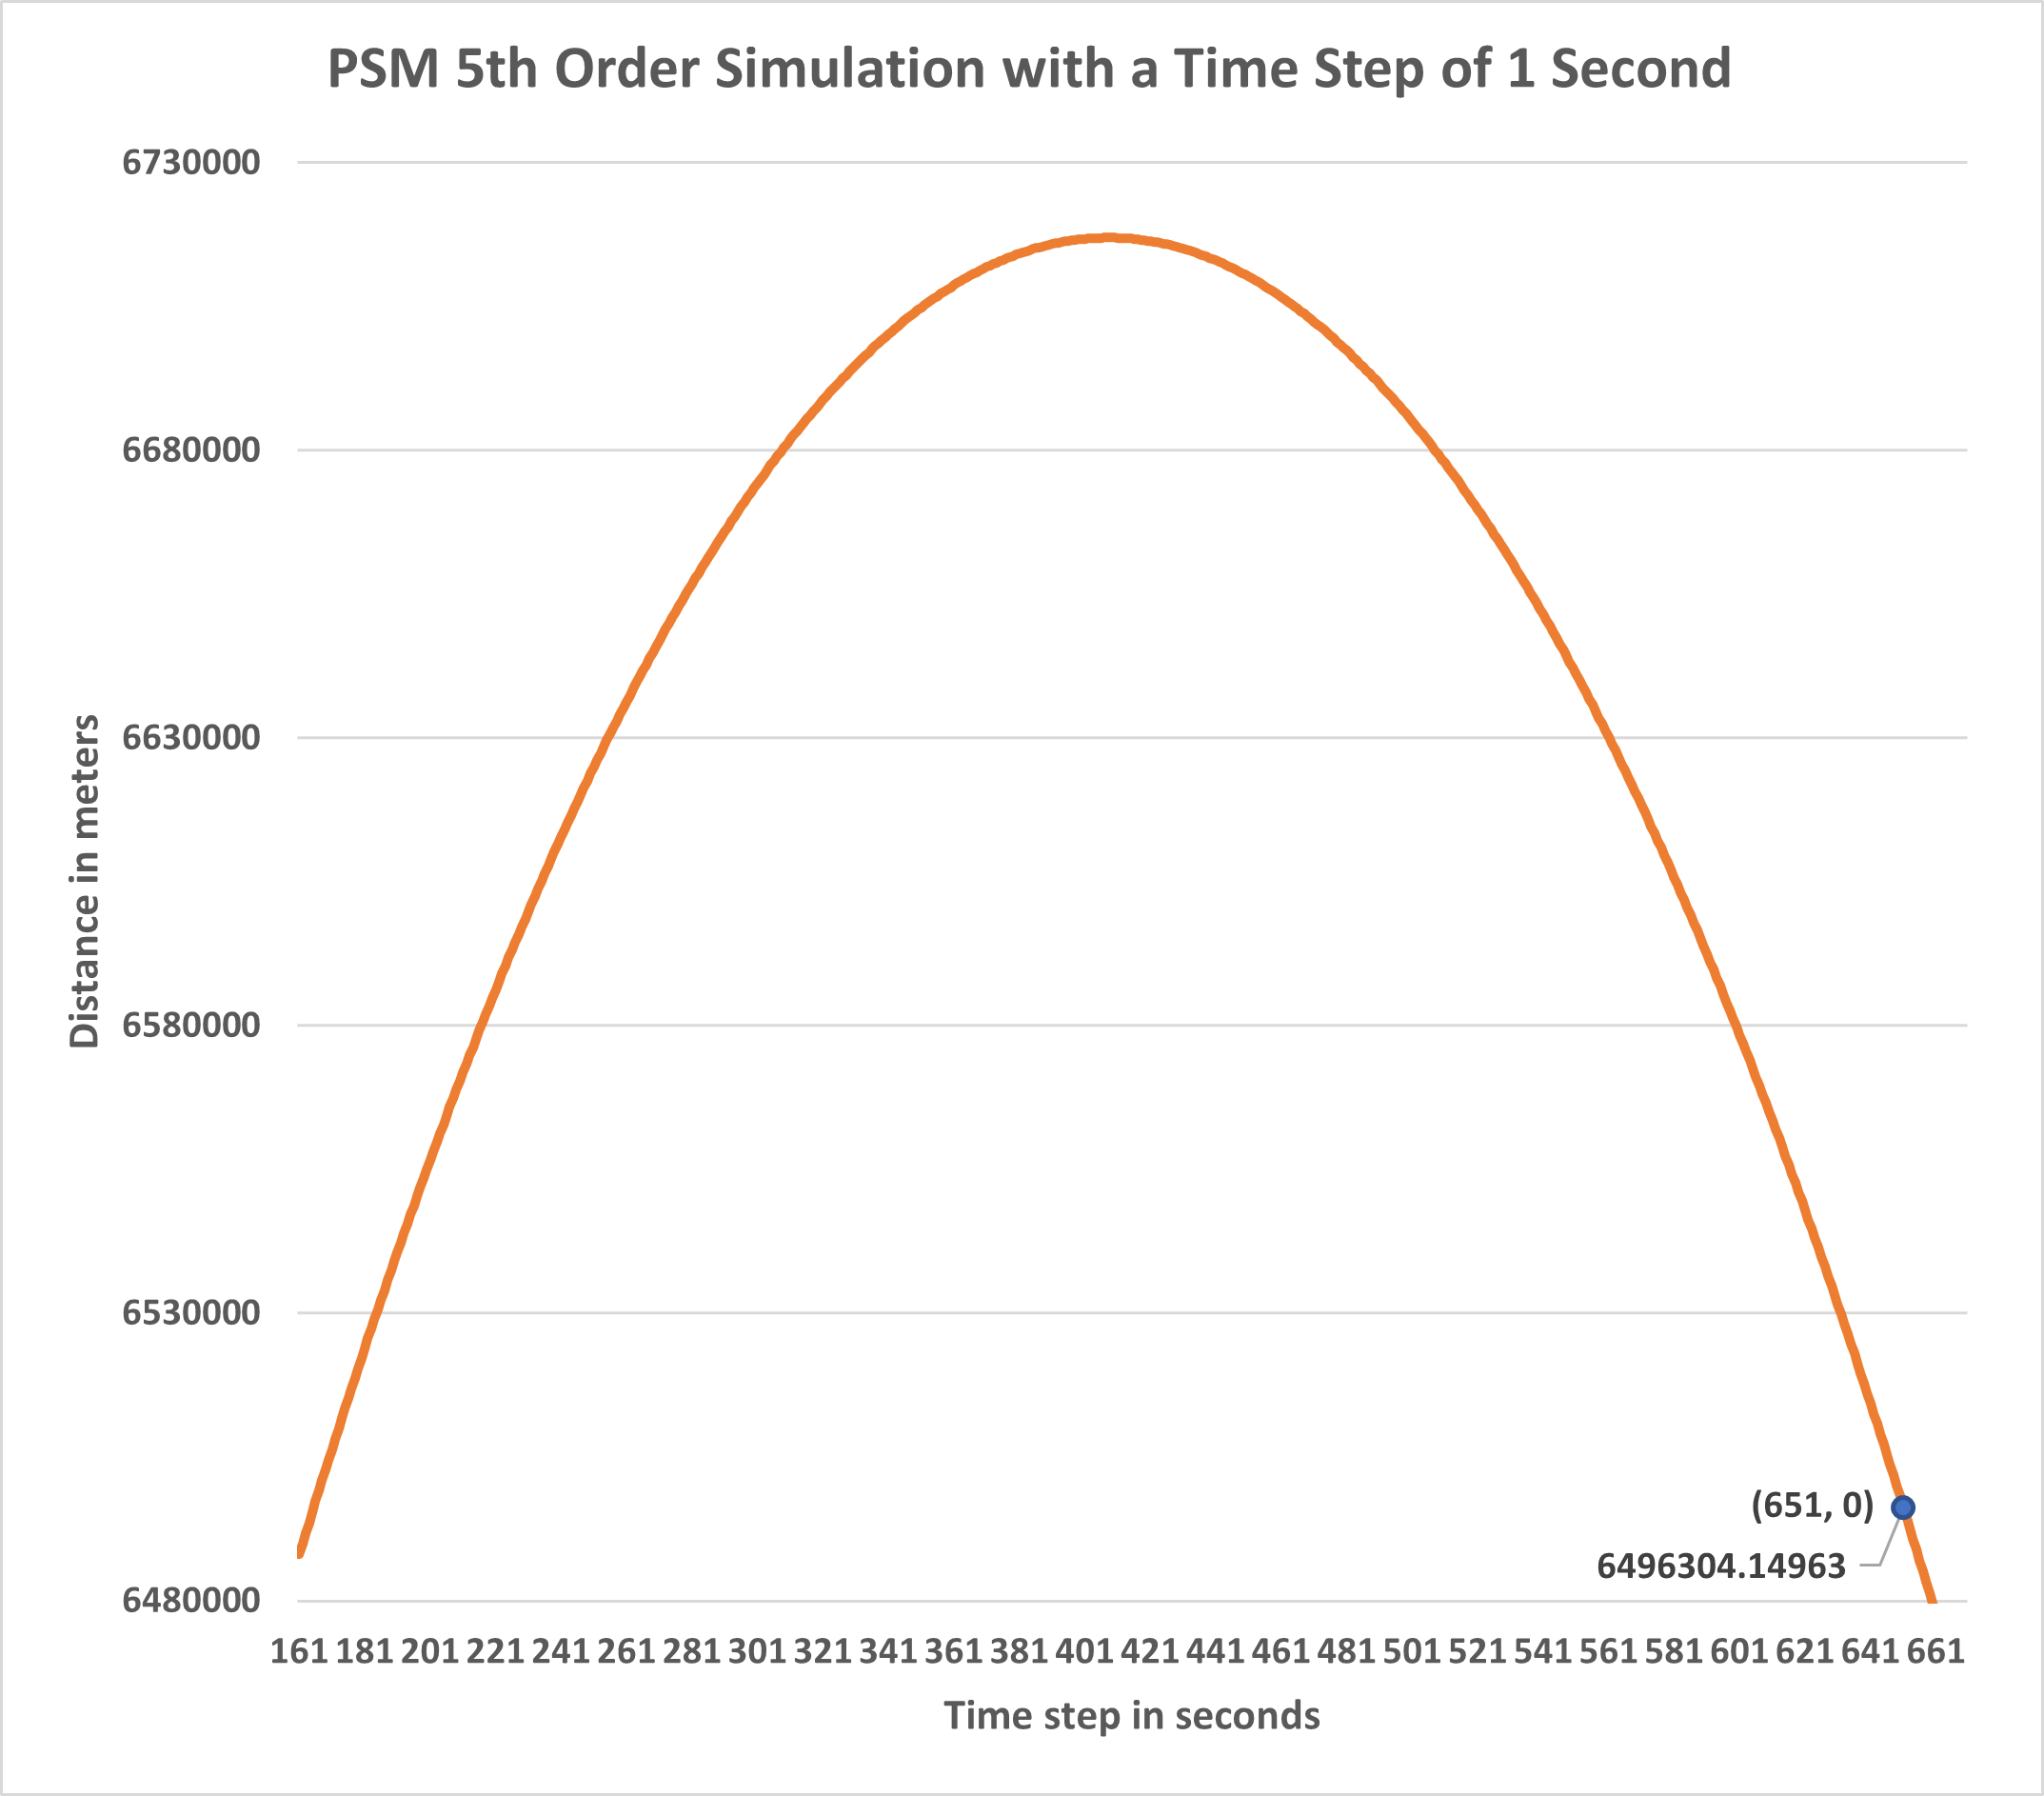
\includegraphics[width=0.22\textwidth]{images/PSM5 TS1 Plot.png}
        \hspace*{1.3cm}
        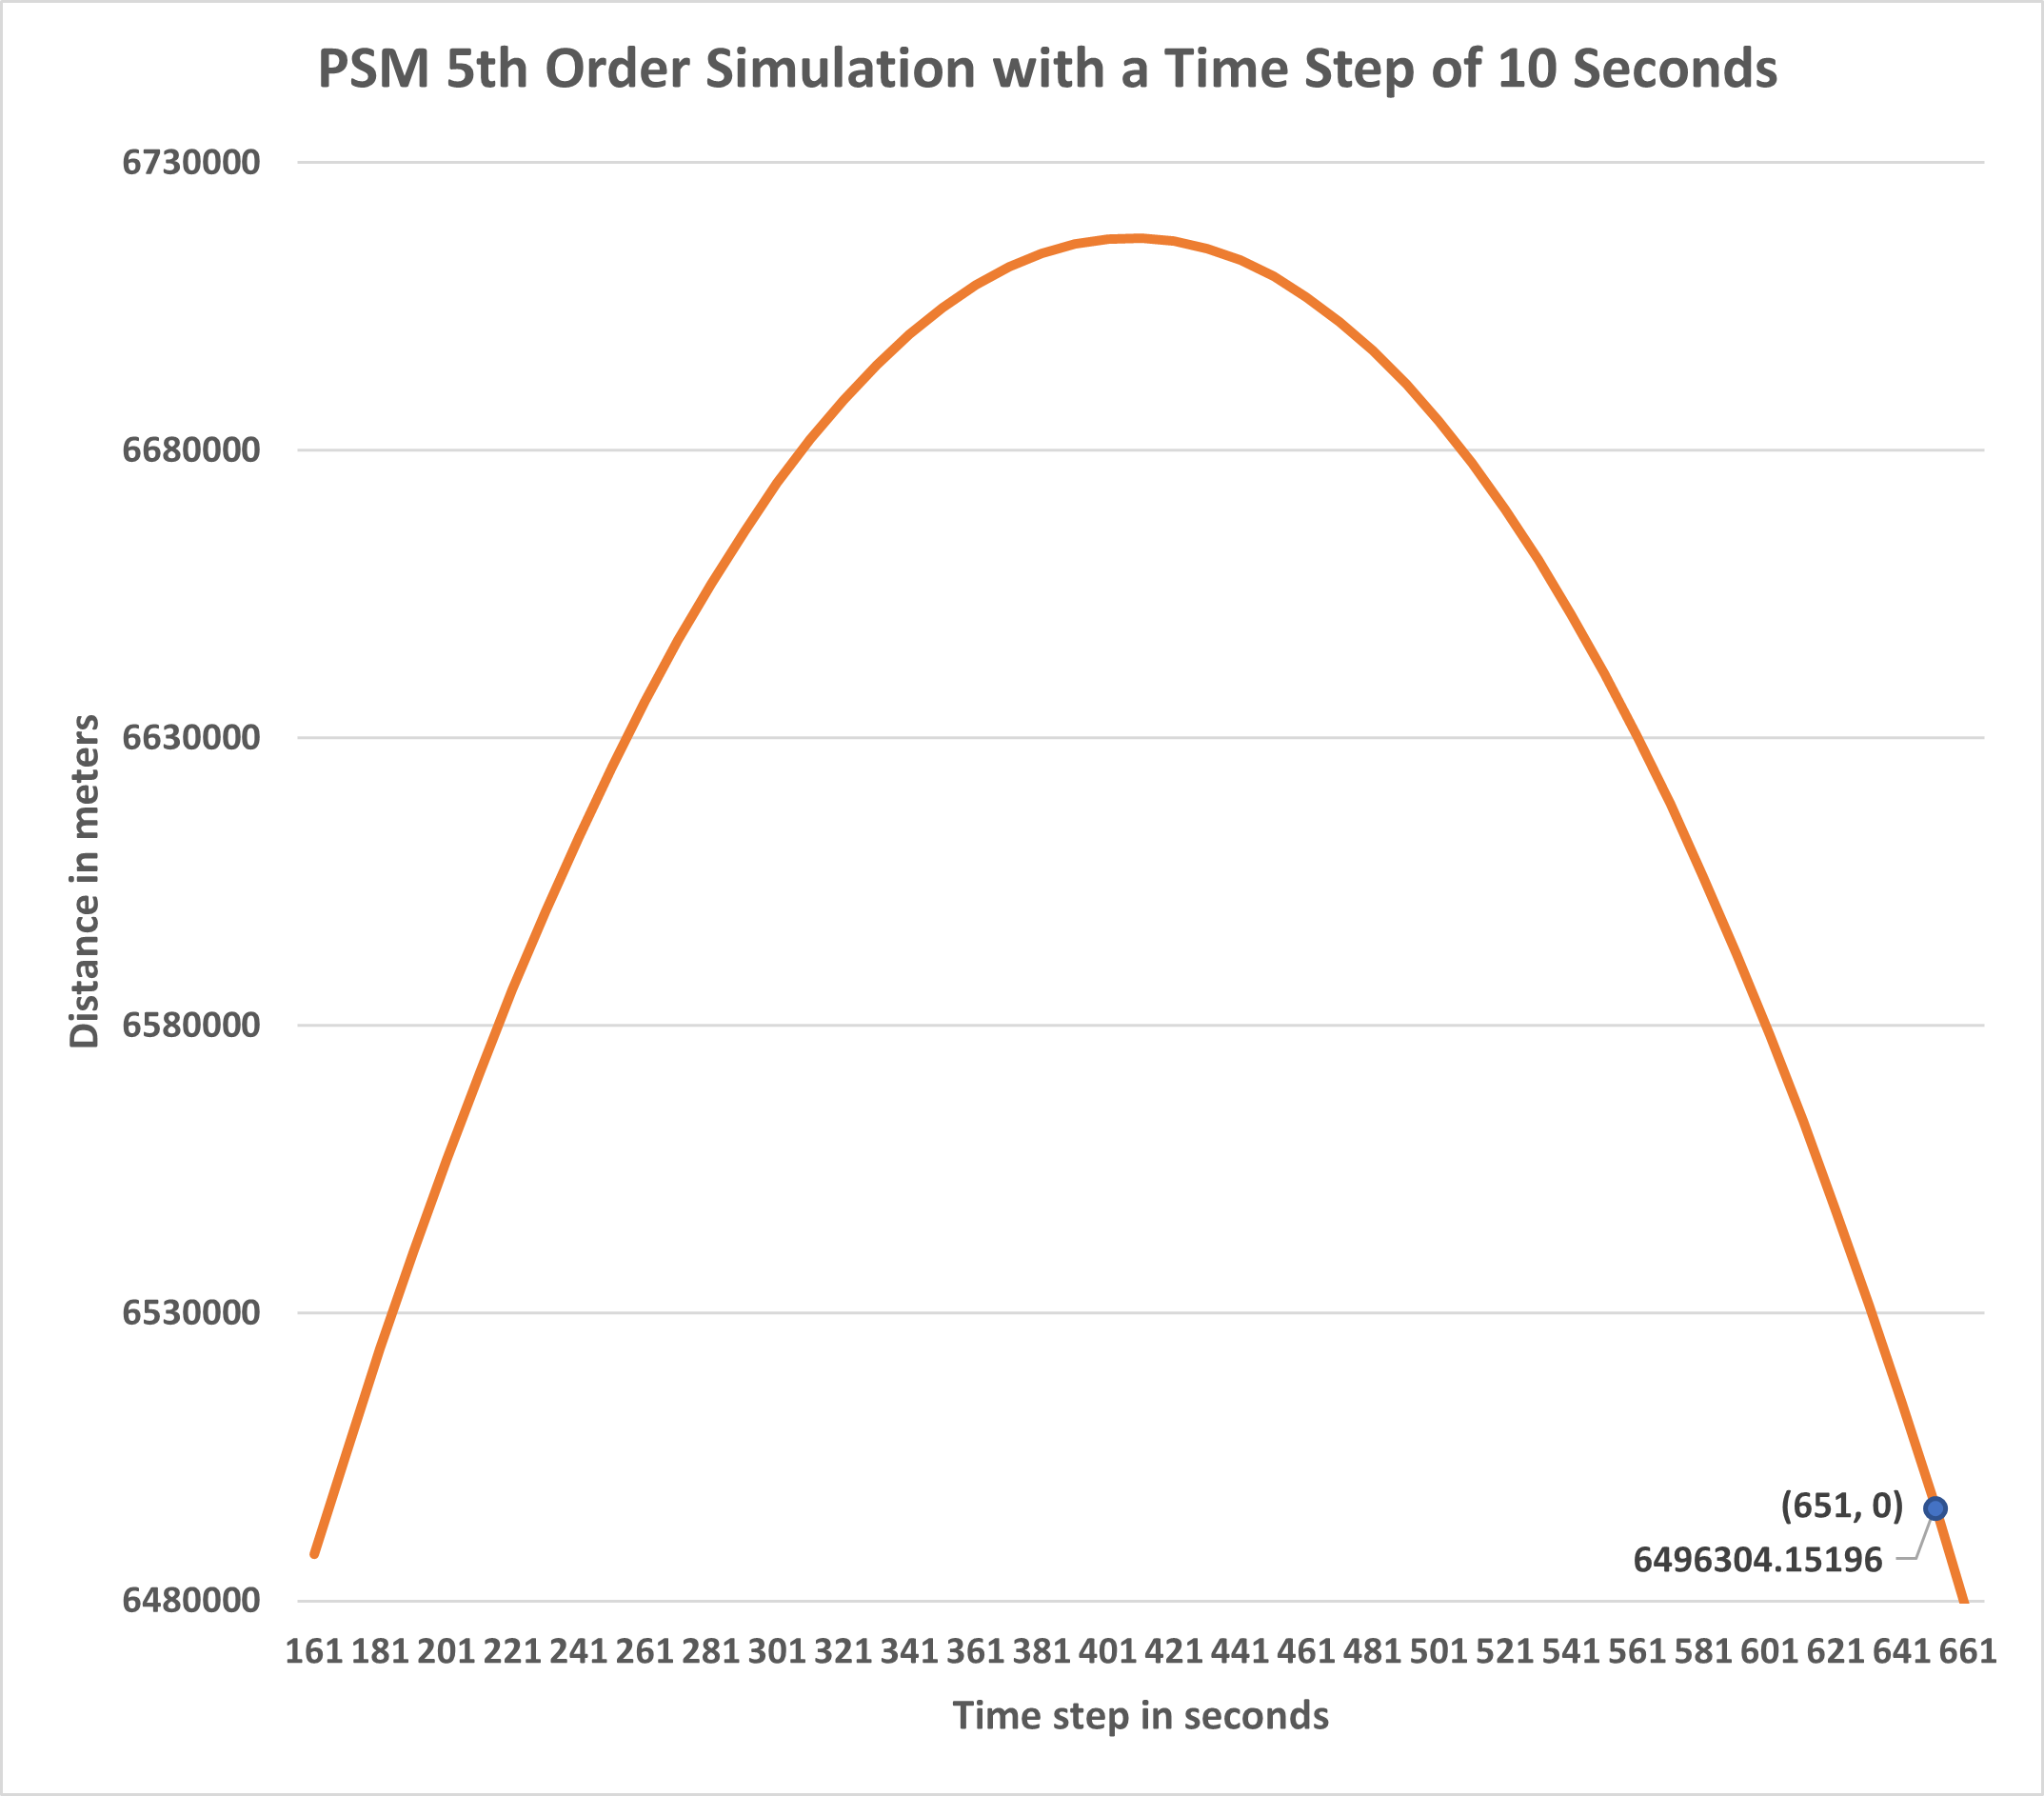
\includegraphics[width=0.22\textwidth]{images/PSM5 TS10 Plot.png}    
        \end{tikzfigure}
        \vspace{.3cm}
        In the plots above, the one on the left is using a time step of 1 and the one on the right
        using a time step of 10.  Labeled, is the point (651, 0), since it is near the end the of
        the plot, where the amount of rounding error is going to be the greatest.  As can be seen, 
        the distance, which is in meters, is only off by less than .01.
    }
    \column{0.45}
    \block{Cauchy Product Example Problem}
    {
        Use the power series method to solve $y^\prime = y^2$ ; $y(0) = -1$
        \begin{equation*}
            y = \sum\limits_{k=0}^{\infty}c_kt^k \Rightarrow y^\prime = \sum\limits_{k=1}^{\infty}kc_kt^{k-1}
        \end{equation*}
        Plug into $y^\prime = y^2$
        \begin{equation*}
            \sum\limits_{k=1}^{\infty}kc_kt^{k-1} = \left(\sum\limits_{k=0}^{\infty}c_kt^k\right) \left(\sum\limits_{k=0}^{\infty}c_kt^k\right)
        \end{equation*}
        Rewrite $y^2$ to match the form of the cauchy product
        \begin{equation}
            \sum\limits_{k=1}^{\infty}kc_kt^{k-1} = \sum\limits_{k=0}^{\infty} \underbrace{\left(\sum\limits_{j=0}^{k}c_jc_{k-j}\right)}_{\text{Cauchy product}}t^k
        \end{equation}
        Set $k = 1$ on both sides of the equation to solve for $c_k$
        \begin{equation*}
            \sum\limits_{k=1}^{\infty}kc_kt^{k-1} = \sum\limits_{k=1}^{\infty} \left(\sum\limits_{j=0}^{k-1}c_jc_{k-j-1}\right)t^{k-1}
        \end{equation*}
        \begin{equation}
            c_k = \frac{\sum\limits_{j=0}^{k-1}c_jc_{k-j-1}t^{k-1}}{k}
        \end{equation}
        Solving for $c_k$, we can see each coefficient is a function of previous coefficients
        \begin{equation*}
            \therefore c_1 = c_0c_0, c_2 = \frac{c_0c_1 + c_1c_0}{2}, c_3 = \frac{c_0c_2 + c_1c_1+ c_2c_0}{3},\dots
        \end{equation*}
    }
    \block{Conclusion}
    {
        PSM is an efficient and highly adaptive way to simulate ballistic missile trajectory.  By 
        plugging in initial conditions of position, velocity, and acceleration, it can accurately 
        simulate the trajectory of a missile in various situations. As can be seen in the graphs and 
        data points, the model works as stated.  The advantage of being able to take larger time 
        steps with PSM compared to RK4 means that any data stored on computers used for solving the 
        simulations are much less, and can be computed faster, while also taking up less space. 
        Overall, PSM can be used in a variety of different applications, as a fast and powerful 
        algorithm.
    }
\end{columns}

\block{References}
{
    \vspace{.5cm}
    All of the source code and references are located on the GitHub repository and can be accessed 
    by scanning the QR code at the top of the poster, or going to the following URL: 
    https://github.com/tierneycolin/ModelingFinalProject 
    \vspace{.5cm}
}

\end{document}